\chapter{Multi-objective problems}
In real world environments, it is current that optimising a cost metric for a target is not sufficient.
Indeed, optimising one metric without considering its consequence on the others should be problematic.
For instance, we should be interested in a strategy that does not fail to reach the target with a cost bounded and that however optimises the expected cost-to-target under this assumption.
Moreover, we should also be interested in getting a strategy satisfying at a time many reachability problems, and furthermore, many shortest path problems. This chapter will cover the resolution of \textit{multi-objective} problems, where we are interested in solving \textit{simultaneously} multiple problems.
\begin{example}[\textit{Communication between nodes in a wireless sensor network}]\label{main-example}
Consider a wireless sensor network containing three nodes $n_0,\, n_1$ and $n_2$. Assume that $n_0, \, n_1$ and $n_3$ are separated by the same distance, that the sensor $n_0$ has to send messages to $n_2$ at regular intervals and that a wall stands between $n_0$ and $n_2$ (cf. Figure \ref{sensor_net}).
\begin{figure}[h!]
  \centering
  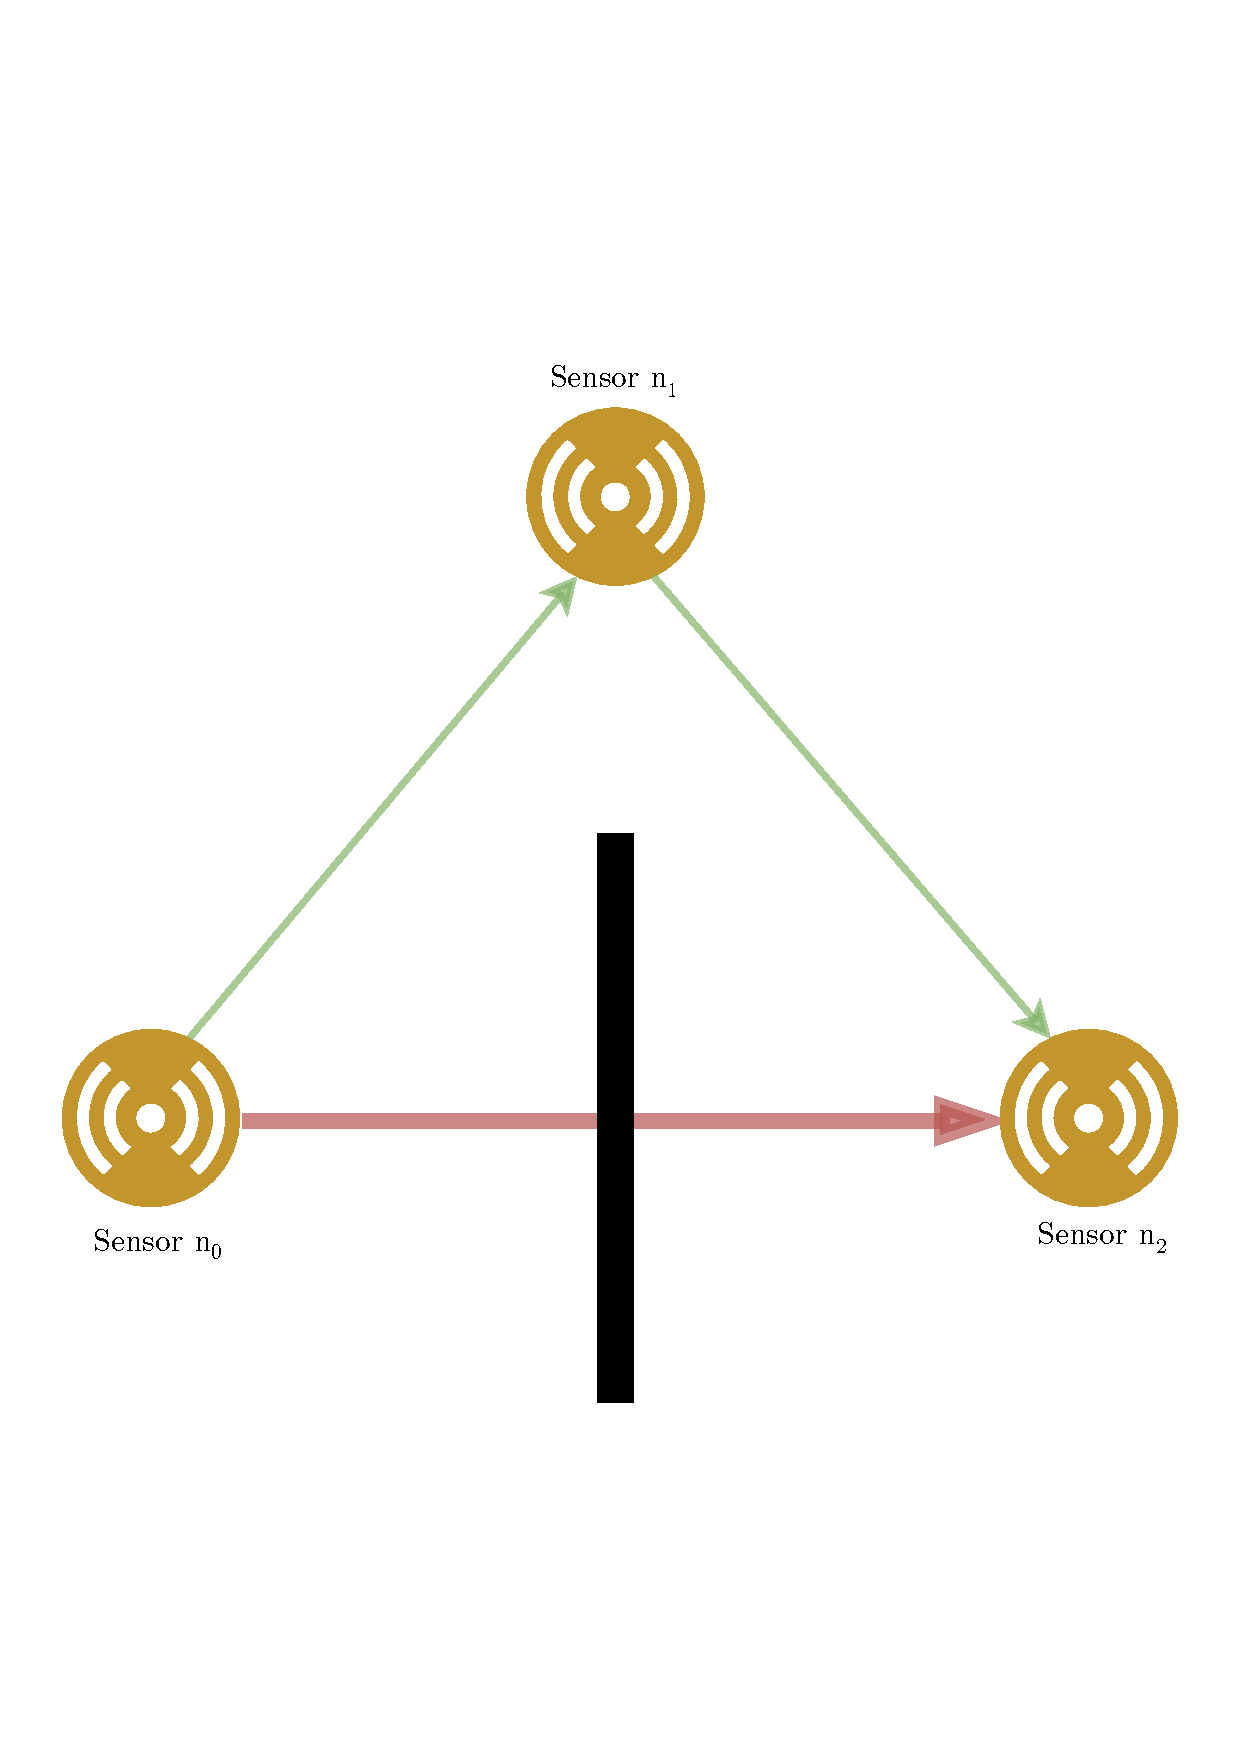
\includegraphics[width=0.7\linewidth]{resources/example3}
  \caption{Communication between three nodes in a wireless sensor network} \label{sensor_net}
\end{figure}
There are two possibilities for $n_0$. First, it can send directly the message to $n_2$. In that case, sending the message is quite quick, but requires more energy that a standard message sending. %(due to the demodulation of a noisy message by $n_2$).
Moreover, this sending has a risk of packet corruption due to the possible noise induced when the signal goes through the wall standing between the two sensors.
The second possibility is to send the message to an intermediate node (i.e., $n_1$). This sending is obviously slower due to the sending in two steps, but requires less energy in total that a direct sending.
In that case, the risk of packet corruption is negligible. \\
This example induces some questions. Firstly, we should be interested by a strategy ensuring a bounded duty cycle for the emitter sensor $n_0$ (i.e., a bounded time for its active state).
Thus, we should be interested by a strategy minimising the expected energy of sending the message while ensuring this duty cycle.
Finally, we should be interested by a strategy offering a good probability to have a bounded duty cycle while having a good probability to minimise the energy used by the sensor to send the message.
\end{example}
\section{Worst case guarantee}
Firstly, we are going to be interested in having a worst case guarantee to reach some states in a Markov decision process, i.e., a guarantee to reach these states with a cost bounded.
To do that, we will approach the problem by considering it as a \textit{shortest path game} problem.
\begin{definition}[\textbf{\SPG{} problem}]
  Let $\mathcal{M}$ be an MDP with state space $S$, $s \in S$, $T \subseteq S$, and $l \in \mathbb{N}$.
  The shortest path game problem (\SPG{}, for short) consists in deciding if there exists a strategy $\sigma$ ensuring to reach the subset of target states $T$ from the state $s$ with a cost bounded $l$, i.e.,
  \begin{align*}
    \forall \pi \in Paths^\sigma(s), \, \TS^T(\pi) \leq l.
  \end{align*}
\end{definition}

\begin{theorem}[\textbf{\textit{\SPG{} problem and qualitative cost bounded reachability}}] \label{spg-thm1}
  Let $\mathcal{M}=(S, A, \Delta, w, AP, L)$ be an MDP, $s \in S$, $T \subseteq S$, $l \in \mathbb{N}$, and $\sigma$ be a strategy on $\mathcal{M}$.
  The following two propositions are equivalent:
  \begin{enumerate}[(a)]
    \item $\forall \pi \in Paths^\sigma(s), \, \TS^T(\pi) \leq l$. \label{qsspp1}
    \item $\mathbb{P}_s^\sigma(\Diamond_{\leq l}\, T) = 1$. \label{qsspp2}
  \end{enumerate}
\end{theorem}
\begin{proof2}$ $\\
  ($\ref{qsspp1}\implies\ref{qsspp2}$). Assume that for all $\sigma$-path $\pi \in Paths^\sigma(s)$, the truncated sum of this path is lower than or equals $l$, i.e., $\TS^T(\pi)\leq l$.
  We have that $\mathbb{P}_s^\sigma(\Diamond_{\leq l}\, T) = \mathbb{P}_s^\sigma(\{ \pi \in Paths(s) \; | \; \TS^T(\pi) \leq l \})$. As all $\sigma$-path starting from $s$ have a truncated sum lower than or equals $l$, we have $\{\pi \in Paths^\sigma(s) \; | \; \TS^T(\pi) \leq l \} = Paths^\sigma(s)$.
  Then, $\mathbb{P}_s^\sigma(\Diamond_{\leq l}\, T) = \mathbb{P}_s^\sigma(Paths(s)) = 1$. \\
  ($\neg \ref{qsspp1} \implies \neg \ref{qsspp2}$). Assume there exists a $\sigma$-path $\pi \in Paths^\sigma(s)$ such that $\TS^T(\pi)>l$. Thus, consider this path $\pi$ and let $\hat{\pi} = s_0\xrightarrow{\alpha_1}\dots \xrightarrow{\alpha_n} s_n \in Pref(\pi)$, where $\alpha_i$ is
  chosen by the strategy $\sigma$ for each $i \in \{1, \dots, n \}$, such that $\sum_{i=1}^n w(\alpha_i) > l$.
  We have $\pi \in Cyl(\hat{\pi})$ and $\mathbb{P}_s^\sigma(Cyl(\hat{\pi})) = \prod_{i=0}^{n-1} \Delta(s_i, s_{i+1}) > 0$.
  We obviously additionally have that $Cyl(\hat{\pi}) \cap \{ \pi \in Paths^\sigma(s) \; | \; \TS^T(\pi) \leq l \} = \emptyset$, because %$s_i \not \in T$ for all $i \in \{0, \dots, n\}$ and
  %$\sum_{i=1}^n w(\alpha_i) > l$.
  $\TS^T(\hat{\pi}) > l$.
  Then, we have
   \[\mathbb{P}_s^\sigma(\Diamond_{\leq l}\, T) = \mathbb{P}_s^\sigma(\{ \pi \in Paths(s) \; | \; \TS^T \leq l \}) \leq 1 - \mathbb{P}_s^\sigma(Cyl(\hat{\pi})) < 1.\]
\end{proof2}
\\

With the theorem \ref{spg-thm1}, it is possible to solve the \SPG{} problem by reduction to the \SSPP{} problem.
However, the \SSPP{} problem is computed in pseudo-polynomial time in $\mathcal{M}$ and in the size of length of $l$, and we want to avoid this class of time complexity.
Here, we consider the MDP as a two players game.
In each step, the system is in state $s$ and the player one chooses an enabled action $\alpha$ of $s$.
Then, the player two chooses the $\alpha$-successor of $s$ leading to the worst case in terms of truncated sum.
Thus, we do not consider probabilities for this problem but rather consider the worst case of choosing each action.
Finding an optimal strategy for the player one allowing to reach $T$ with a cost less than or equals $l$
under the choices of the player two solves the \SPG{} problem. \\

We compute the shortest path in this game from $s$ to $T$ by dynamic programming in order to build a strategy solving the \SPG{} problem.
Let $|S| = n$ and $\mathbb{C}: S \times \{0, \dots, n-1 \}$ be a function such that $\mathbb{C}(s, i)$ is the shortest path from $s$ to $T$ in this game after maximum
$i$ playing steps.
Obviously, $\mathbb{C}$ can be represented with a matrix of size $n \times n$.
We have \[\mathbb{C}(s, 0) = \begin{cases}
  0 & \text{if } s \in T\\
  +\infty & \text{else}.
\end{cases}\]
Thus, let $k \in \mathbb{N}$, such that $0 \leq k < n - 1$,
\[
  \mathbb{C}(s,\, k+1) = \min \big[\mathbb{C}(s,\, k),\, \min_{\alpha \in A(s)} \max_{s' \in Succ(s,\alpha)} \big(w(\alpha) + \mathbb{C}(s',\, k)\big)\big].
\]
This recursive definition of $\mathbb{C}$ actually means that the shortest path from $s$ to $T$ in maximum $k+1$ steps corresponds to either the shortest path from $s$ to $T$ in maximum $k$ steps or the minimal weight of choosing an action $\alpha$ plus the shortest path from the worst $\alpha$-successor $s'$ of $s$ to $T$ in maximum $k$ steps.
\begin{figure}[h]
  \centering
  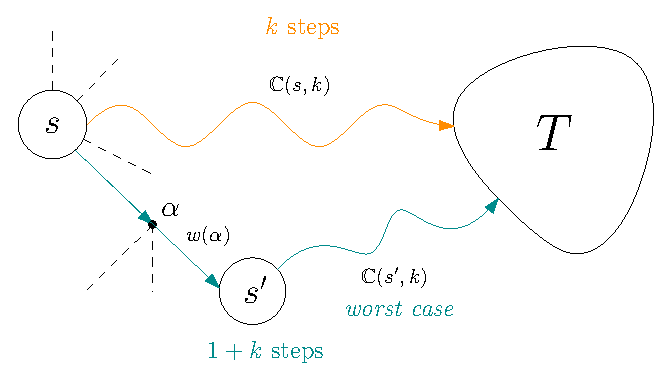
\includegraphics[width=0.6\linewidth]{resources/sp-g}
  \captionsetup{justification=centering}
  \caption{Intuitive representation of  the function $\mathbb{C}$ to solve the \SPG{} problem}
\end{figure}
The minimisation term according to an action in this definition corresponds to the choice of the strategy (i.e., the player one).
The maximisation term in this definition corresponds to the adversary (i.e., the player two), choosing the worst $\alpha$-successor of $s$.
As the weight of each action is strictly positive, the strategy never chooses an action leading to a cycle in this game if it is possible to avoid it.
Then, choosing an action leading to a cycle necessarily yields an infinite truncated sum, and if a strategy satisfying this problem exists, it wins in at most $n - 1$ steps. It is why we only need to consider the $n$ first steps.

\begin{theorem}[\textit{\textbf{Solving the \SPG{} problem}}] The \SPG{} problem can be decided in polynomial time in the size of $\mathcal{M}$ and % with the recursive function $\mathbb{C}$ (and more precisely in $\mathcal{O}(n^2)$ with memoization).
an optimal pure memoryless strategy always exists.% and can also be built in $\mathcal{O}(n^2)$.
\end{theorem}

By dynamic programming, we can determine all values of $\mathbb{C}$ for all entries $(s, i) \in S \times \{0, \dots, n-1\}$ with a time complexity in $\mathcal{O}(n^2)$.
Let $s$ be a state of the MDP. By definition of $\mathbb{C}$, we have $\mathbb{C}(s,\, k + 1) \leq \mathbb{C}(s,\, k)$, for all $k \in \mathbb{N}$ such that $0 \leq k < n-1$.
Then, we have $\mathbb{C}(s, \, n-1) = \min_{k} \mathbb{C}(s, \, k)$, and
a strategy satisfying the \SPG{} problem for $s \in S$ exists if and only if $\mathbb{C}(s,\, n-1) \leq l$.
Furthermore, we can build this pure memoryless strategy as follows:
\[
  \sigma : S \rightarrow A, \; s \mapsto \arg \min_{\alpha \in A(s)} \big[ \max_{s' \in Succ(s, \alpha)} \big(w(\alpha) + \mathbb{C}(s',\, n - 1) \big) \big].
\]
The key idea behind this definition is that $\sigma$ will choose the action minimising the weight of the enabled actions plus the smallest cost to reach $T$ in this game from the worst successor, chosen by the player two.

\begin{remark}[\textit{\SPG{} problem and PRCTL model checking}]
  Let $\mathcal{M}=(S, A, \Delta, w, AP, L)$ be an MDP, $s \in S$, $l \in \mathbb{N}$, and $\Phi$ be a PRCTL state formula over $AP$,
  verify $s \models \mathcal{P}^{\max}_{=1}(\Diamond_{\leq l}\, \Phi)$ is equivalent to solve the \SPG{} problem for the state $s$, the cost threshold $l$ and the subset of target states $Sat(\Phi)$.
\end{remark}

\begin{example}[\textit{\SPG{} problem in the wireless sensor network}] \label{spg-example}
Get back to Example \ref{main-example}.
For this example, we will only consider the time dimension to model the situation.
We focus on the behaviour of the node $n_0$  (cf. Figure \ref{sensor_net_mdp}).
When $n_0$ becomes active, it has to send a message to $n_2$. We assume here that a standard message sending takes $2$ \textit{mili seconds} ($ms$). If $n_0$ decides to send the message passing by $n_1$, it must wait to receive an acknowledgement of the message sent from $n_1$ to $n_2$. We assume that an acknowledgement message take $2$ $ms$ to be received.
Thus, we have that $n_0$ sends the message to $n_1$ ($2$ $ms$), then $n_1$ sends the message to $n_2$ ($2$ $ms$). When $n_2$ receives the message, it sends an acknowledgement to $n_1$ ($2$ $ms$) and $n_1$ sends an acknowledgement to $n_0$ ($2$ $ms$).
Then, after that $n_0$ has sent the message to $n_1$, he waits $6$ $ms$ the acknowledgement from $n_1$ and go to sleep during $10$ $ms$ after that. If $n_0$ decides to directly send a message to $n_2$, then $n_2$ sends the message and waits $2$ $ms$ the acknowledgement.
Due to the possible packet corruption, $n_2$ does not receive the acknowledgement with a probability $\frac{1}{8}$. In that case, it has to try sending the message again.
Else, it goes to sleep during $10$ $ms$.
\begin{figure}[h]
  \centering
  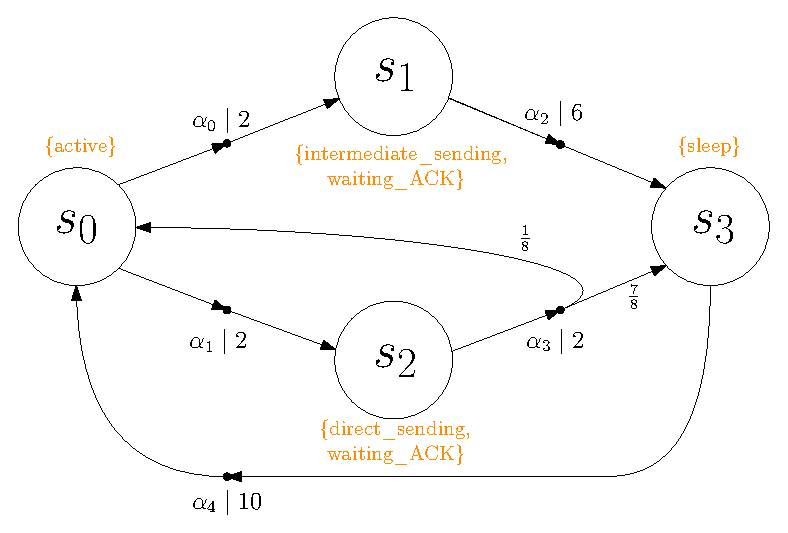
\includegraphics[width=0.6\linewidth]{resources/example3.eps}
  \captionsetup{justification=centering}
  \caption{MDP representing the behaviour of the node $n_0$, according to the situation of Figure \ref{sensor_net} from Example \ref{main-example}}\label{sensor_net_mdp}
\end{figure}

Assume we want to ensure a duty cycle of $12$ $ms$ for the node $n_0$. Then, let $\mathcal{M}=(S, A, \Delta, w, AP, L)$ be the MDP of Figure \ref{sensor_net_mdp}, we want to solve the following \SPG{} problem:
\[
  s_0 \overset{?}{\models} \, \mathcal{P}^{\max}_{=1}(\Diamond_{\leq 12} \; \textit{sleep}).
\]
To solve this problem, we will recursively compute $\mathbb{C}$ for all $s \in S$ from $k=0$ to $k=3$:
\begin{minipage}{0.5\linewidth}
    \begin{itemize}
      \item[$k=0$] \begin{itemize}
[label=\raisebox{0.25ex}{\tiny$\bullet$}]        \item $\mathbb{C}(s_0, 0) = \mathbb{C}(s_1, 0) = \mathbb{C}(s_2, 0) = +\infty$
        \item $\mathbb{C}(s_3, 0) = 0$
      \end{itemize}
      \item[$k=1$]
        \begin{itemize}
[label=\raisebox{0.25ex}{\tiny$\bullet$}]          \item $\mathbb{C}(s_0, 1) = +\infty$
          \item $\mathbb{C}(s_1, 1) = 6 + 0 = 6$
          \item $\mathbb{C}(s_2, 1) = 2 + \infty = +\infty$
        \end{itemize}
      \item[$k=2$]
        \begin{itemize}
[label=\raisebox{0.25ex}{\tiny$\bullet$}]          \item $\mathbb{C}(s_0, 2) = 2 + 6 = 8$
        \end{itemize}
      \item[$k=3$]
        \begin{itemize}
[label=\raisebox{0.25ex}{\tiny$\bullet$}]          \item $\mathbb{C}(s_2, 3) = 2 + 8 = 10$
        \end{itemize}
    \end{itemize}
\end{minipage}
\begin{minipage}{0.5\linewidth}
\centering
\begin{tabular}{l|llll}
$S$ & $k=0$     & $k=1$     & $k=2$     & $k=3$ \\ \hline
$s_0$  & $+\infty$ & $+\infty$ & 8         & 8     \\
$s_1$  & $+\infty$ & 6         & 6         & 6     \\
$s_2$  & $+\infty$ & $+\infty$ & $+\infty$ & 10    \\
$s_3$  & 0         & 0         & 0         & 0
\end{tabular}
\captionsetup{justification=centering}
\captionof{table}{Computing $\mathbb{C}$ by dynamic programming}
\end{minipage}
\\$ $\\$ $\\
The result $\mathbb{C}(s_2,3)=10$ is interesting. It means that the player one firstly chooses the action $\alpha_3$ (with a weight of $2$).
Then, the player two chooses worst case, i.e., the transition $s_2 \xrightarrow{\alpha_3}s_0$, and the player one next chooses the action surely leading $s_0$ to $s_3$ with a minimal cost (i.e., $\mathbb{C}(s_0, 2)=8$ with $s_0\xrightarrow{\alpha_0}s_1\xrightarrow{\alpha_2}s_3$).
\par As $\mathbb{C}(s_0,\, 3) \leq 12$, the duty cycle is ensured by the strategy built with $\mathbb{C}$, and we have $s_0 \models \mathcal{P}^{\max}_{=1}(\Diamond_{\leq 12}\; \textit{sleep})$.
With this strategy, the sensor $n_0$ will always choose to send the message via $n_1$.
This ensures a duty cycle of $8$ $ms$, but it is possible to have a better expected time to reach the \textit{sleep} state (e.g., with a memory strategy).
Thus, the next type of strategy that we will study is strategies offering a good expected cost-to-target while ensuring to reach this target with a cost bounded.
\end{example}

\section{Good expectation under a worst case}
We will now study strategies ensuring simultaneously a worst case threshold (cf. previous section) and a good expected cost-to-target in a Markov decision process.

\begin{definition}[\textbf{\SSPWE{} problem}]
    Let $\mathcal{M}=(S, A, \Delta, w, AP, L)$, be an MDP, $s \in S$, $T \subseteq S$, and $l_1, l_2 \in \mathbb{N}$.
    The \textit{stochastic shortest path worst case expectation} problem (\SSPWE{}, for short) consists in deciding if there exists a strategy $\sigma$ such that:
    \begin{itemize}
      \item $\forall \pi \in Paths^\sigma(s), \; TS^T(\pi) \leq l_1$.
      \item $\mathbb{E}_s^\sigma(\TS^T) \leq l_2$.
    \end{itemize}
\end{definition}

The \SSPWE{} problem is thus a \textit{multi-objective} problem: indeed, we want actually to solve simultaneously the \SPG{} problem and the \SSPE{} problem.
As a reminder, in the previous section we have replaced the probabilities by an adversarial choice to handle the guarantee to reach a set of target states respecting a worst case.
Here, we will combine this approach with taking into account probabilities for the expected cost-to-target part.
Although the \SSPE{} and the \SPG{} problems can both be decided in polynomial time, the \SSPWE{} is more complex due to the strategy having to satisfy both problems at the same time.

\begin{definition}[\textbf{Attractor of a set of target states in an MDP}]
  Let $\mathcal{M}$ be an MDP with state space $S$ and $T \subseteq S$. The set of \textit{attractors} of $T$ is the set of states reaching $T$ with a maximum probability one, i.e., the set $\{ s \in S \; | \; \mathbb{P}^{\max}_s (\Diamond T) = 1 \}$.
\end{definition}

Let $\mathcal{M}=(S, A, \Delta, w, AP, L)$ be an MDP, the \SSPWE{} problem for $\mathcal{M}$, the state $s \in S$, the subset of target states $T \subseteq S$, and the cost thresholds $l_1, l_2 \in \mathbb{N}$ can be solved with the following algorithm:
\begin{enumerate}
  \item We compute the unfolding of $\mathcal{M}$ from $s$ up to the cost threshold $l_1$, i.e., $\mathcal{M}_{l_1}$ with state space $S_{l_1}$.
  %\item We compute $\mathbb{A}: S \times \{0, \dots, l_1\} \cup \{\bot\} \rightarrow A$, for each state of $S_{l_1}$, yielding the set of \textit{safe actions} allowing to surely go to a successor being in the set of attractors of $T_{l_1} = \{ (s, v) \in S_{l_1} \; | \; s \in T \, \wedge \, v \leq l_1 \}$.
  \item Then, we compute the set of \textit{safe actions} allowing each state in $S_{l_1}$ to surely go to a successor being in the set of attractors of
  $T_{l_1} = \{ (s, v) \in S_{l_1} \; | \; s \in T \, \wedge \, v \leq l_1 \}$.
  More formally, we compute \[\mathbb{A}: S_{l_1} \rightarrow 2^A, \, (s, v) \mapsto \{ \alpha \in A(s) \; | \; \forall (s', v') \in Succ((s, v), \, \alpha), \, \mathbb{P}^{\max}_{(s', v')}(\Diamond T_{l_1}) = 1 \}\]
  for all states $(s, v) \in S_{l_1}$. Thus, for each state $(s, v) \in S_{l_1}$, $\mathbb{A}(s, v)$
  is the set of actions $\alpha \in A(s)$ ensuring to reach $T_{l_1}$ from $(s, v)$ regardless of the evolution of $\mathcal{M}_{l_1}$ by the uncertainty associated with the probabilities.
  \item Next, we compute $\mathcal{M}^\mathbb{A}_{l_1}$, the unfolding of $\mathcal{M}$ up to $l_1$ restricted by the set of attractors of $T_{l_1}$. The key idea is that we remove the states $(s, v)$ such that $\mathbb{A}(s, v) = \emptyset$ from $\mathcal{M}_{l_1}$. More formally,
  we define $\mathcal{M}^\mathbb{A}_{l_1} = (S^\mathbb{A}_{l_1}, \mathbb{A}^*, \Delta^*_{l_1}, w, AP, L_{l_1})$ as follows:
  \begin{itemize}
    \item $S^\mathbb{A}_{l_1} = \{ (s, v) \in S_{l_1} \; | \; \mathbb{A}(s, v) \neq \emptyset \, \vee \, (s, v) \in T_{l_1} \}$,
    \item $\mathbb{A}^* = A$, and the set of enabled actions of each state $(s, v) \in S^\mathbb{A}_{l_1}$ is given by %$\mathbb{A}(s, v)$ if $\mathbb{A}(s, v) \neq \emptyset$ and a singleton containing an arbitrary action $\alpha \in A(s)$ else,
    \[
      \mathbb{A}^*(s, v) = \begin{cases}
        \mathbb{A}(s, v) & \text{if } \mathbb{A}(s, v) \neq \emptyset, \, \\
        \{\alpha\}, \; \text{where } \alpha \in A(s) & \text{else},
      \end{cases}
    \]
    \item $\Delta^*_{l_1}$ is defined as for the classical unfolding $\mathcal{M}_{l_1}$, except for $(s, v)$ such that $\mathbb{A}(s, v) = \emptyset$, where $\Delta^*_{l_1}((s, v),\, (s, v)) = 1$ and $\Delta^*_{l_1}((s, v), \, (s', v')) = 0$ if $(s', v') \neq (s, v)$.
    \item $w, \, AP, \, L_{l_1}$ are defined as for the classical unfolding $\mathcal{M}_{l_1}$.
  \end{itemize}
  Note that we define $\mathbb{A}^*$ and $\Delta_{l_1}^*$ this way because we must handle the case of $(s, v) \in T_{l_1}$ and $\mathbb{A}(s, v) = \emptyset$.
  \item Finally, we solve the \SSPE{} problem in $\mathcal{M}^\mathbb{A}_{l_1}$ for the state $(s, 0)$, the subset of target states $T_{l_1}$, and the cost threshold $l_2$.
\end{enumerate}
Let $(s, v) \in S_{l_1}$, the set of safe actions of $(s, v)$, i.e., $\mathbb{A}(s, v)$, can be computed recursively
% with the function $\mathbb{A}_i$, for $i \in \mathbb{N}$, %corresponding to the set of actions ensuring to reach a \textit{safe state} in $i$ steps (i.e., a state in the set of attractors of $T_{l_1}$),
%that is defined
as follows:
\[
  \mathbb{A}_0(s, v) = \begin{cases}
    A(s) & \text{if }v \leq l_1,\\
    \emptyset & \text{else},
  \end{cases}
\]
then, let $i \in \mathbb{N}$, assume that $\mathbb{A}_i$ has already been computed,
\[
  \mathbb{A}_{i+1}(s, v) = \{ \alpha \in \mathbb{A}_i(s, v) \; | \;
    \forall (s', v') \in Succ( (s, v), \alpha ) \setminus T_{l_1}, \; \mathbb{A}_i(s', v') \neq \emptyset \}.
\]
%The key idea behind this definition is that
%$\mathbb{A}_i(s,v)$ is the set of enabled actions of $(s, v)$ ensuring to not reach a \textit{bad state} in at most $i$ transitions.
The key idea behind this definition of $\mathbb{A}_i$ is that we inductively disable the unsafe enabled actions of all states.
We consider that a state that has no more enabled action is a \textit{bad state}.
At the initialisation, i.e., at $i=0$, all enabled actions of each state are safe except if the current cost of a state has exceeded the threshold $l_1$. In that case, this state is a bad state.
%Then, we inductively consider the successors  of $(s, v)$ reachable in $i$ steps from the current state $(s, v)$ and inductively remove the enabled actions of $(s, v)$ ensuring to reach a bad states from one of these successors, in at most $i$ steps.
%Then, we inductively increase the scope of successors considered up to a \textit{bad state}, i.e., a state exceeding the cost $l_1$. Each action
By induction, at each step and for each state $(s, v)$,
%By induction, at the step $i$,
we disable the actions $\alpha$
%of each state
that risk to lead $(s, v)$ to one of its $\alpha$-successor considered as a bad state.% in at most $i$ transitions.
\begin{figure}[h]
  \begin{minipage}{0.5\linewidth}
    \centering
    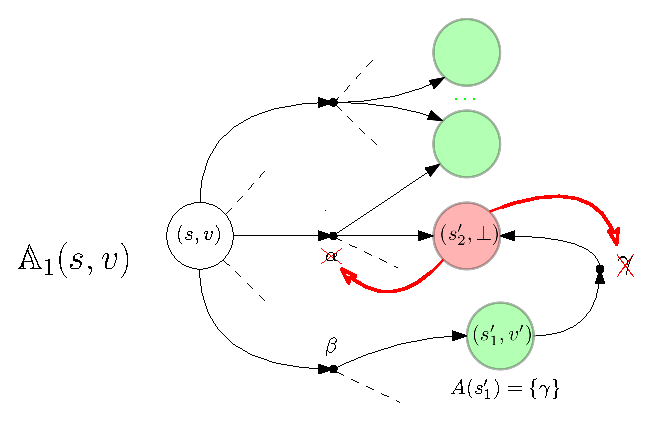
\includegraphics[width=0.9\linewidth]{resources/attractor}
  \end{minipage}
  \begin{minipage}{0.5\linewidth}
    \centering
    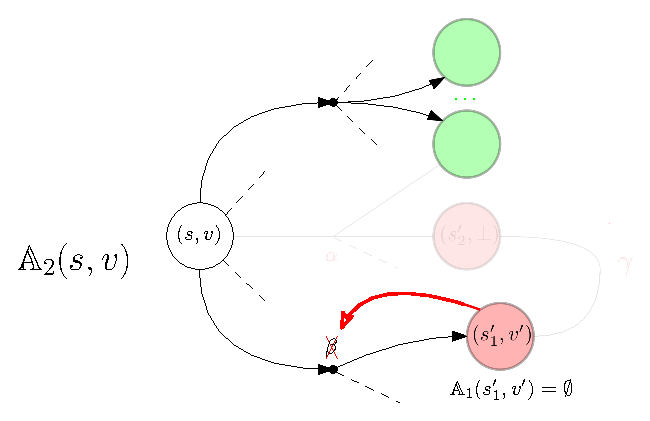
\includegraphics[width=0.9\linewidth]{resources/attractor2}
  \end{minipage}
  \caption{Intuition of the recursive computation of $\mathbb{A}$}
\end{figure}

The way we compute $\mathbb{A}$ is actually the same
as when we compute the largest set $S_{=1} = \{ s \in S \; | \; \mathbb{P}^{\max}_s(\Diamond T) = 1 \}$ (cf. algorithm \ref{prMax1} from Appendix \ref{LP-app}).
Computing $\mathbb{A}$ this way particularises the algorithm \ref{prMax1} for $\mathcal{M}_{l_1}$ to only keep the actions leading to attractors of $T_{l_1}$, in order to build $\mathcal{M}^\mathbb{A}_{l_1}$ and solve the \SSPE{} problem in it.

\begin{theorem}[\textbf{\textit{Solving the \SSPWE{} problem}}]
  The \SSPWE{} problem can be decided in pseudo-polynomial time in the size of $\mathcal{M}$ and in the size of the length of $l_1$.
  Pure pseudo-polynomial memory strategies satisfying this problem can be built in pseudo-polynomial time in the size of $\mathcal{M}$ and in the size of the length of $l_1$.
\end{theorem}

By definition, the size of the set $\mathbb{A}_i$ is decreasing with $i$, i.e., for all $i \in \mathbb{N}$,
\[
  | \mathbb{A}_i | \geq | \mathbb{A}_{i+1} |.
\]
By construction, the underlying graph of the unfolding of $\mathcal{M}$ up to $l_1$ is a directed acyclic graph (i.e., a DAG). Moreover, the weight of each action is a strictly positive integer. Then, there is no cycle in $\mathcal{M}_{l_1}$ and each state reach $T_{l_1}$ in at most $l_1$ transitions (this worst case corresponds to the case of $w(\alpha)=1$ for all $\alpha \in A$).
The time complexity of the construction of $\mathbb{A}$ is thus polynomial in the size of $\mathcal{M}_{l_1}$ (more precisely in $\mathcal{O}(l_1 \times |S_{l_1}|) = \mathcal{O}(l_1^2 \times |S|)$), and is thus pseudo-polynomial in the size of $\mathcal{M}$ and in the size of the length of $l_1$. Then, as solving the \SSPE{} problem in $\mathcal{M}^\mathbb{A}_{l_1}$ is polynomial in the size of $\mathcal{M}^\mathbb{A}_{l_1}$,
the entire algorithm presented to solve this problem is pseudo-polynomial in the size of $\mathcal{M}$ and in the size of the length of $l_1$.
Furthermore, as the strategy solving the \SSPE{} problem in $\mathcal{M}_{l_1}^\mathbb{A}$ is memoryless in $\mathcal{M}_{l_1}^\mathbb{A}$, it requires pseudo-polynomial memory in $\mathcal{M}$ (intuitively, the strategy has $l_1 + 1$ modes).

\begin{example}[\textit{\SSPWE{} problem in the wireless sensor network}]
  Again, get back to Example \ref{main-example}.
  We consider the MDP $\mathcal{M}$ of Figure \ref{sensor_net_mdp}. As in Example \ref{spg-example}, we are interested by a strategy ensuring a duty cycle of $12$ $ms$ for the node $n_0$, but at the same time ensuring a minimal expected time to reach the \textit{sleep} state, allowing it to go to sleep as soon as possible.
  Assume that we are interested by the following \SSPWE{} problem:
  \[
    ?\exists \sigma \; \;  \mathbb{P}^\sigma_{s_0}(\Diamond \{s_2\}) \leq 12 \; \wedge \; \mathbb{E}^\sigma_{s_0}(\TS^{\{s_2\}}) \leq 6,
  \]
  where $6$ $ms$ is half the time of the duty cycle that we want to ensure. First, we begin by unfolding $\mathcal{M}$ from $s_0$ up to the cost threshold $12$ (cf. Figure \ref{unfolding-sspwe}), yielding the MDP $\mathcal{M}_{l_1}$.
  \begin{figure}[h]
    \centering
    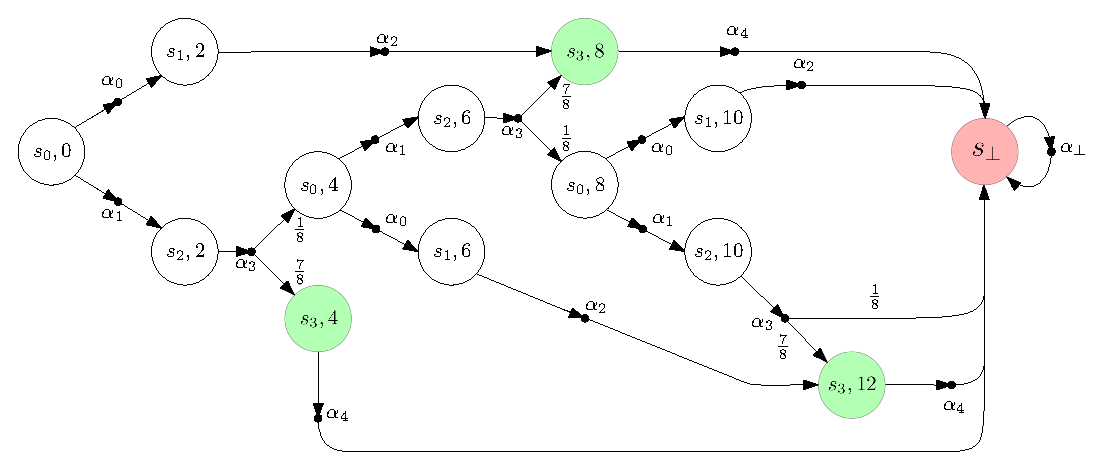
\includegraphics[width=0.9\linewidth]{resources/main-example-unfolding}
    \captionsetup{justification=centering}
    \caption{Unfolding of $\mathcal{M}$ (cf. Figure \ref{sensor_net_mdp}) from $s_0$ (i.e., from the active state) up to $12$ $ms$}
    \label{unfolding-sspwe}
  \end{figure}
  \begin{table}[h]
  \centering
\begin{tabular}{l|cccccc}
$S_{12}$          & \multicolumn{1}{l}{$i=0$} & \multicolumn{1}{l}{$i=1$}                                  & \multicolumn{1}{l}{$i=2$}  & \multicolumn{1}{l}{$i=3$}  & \multicolumn{1}{l}{$i=4$} & \multicolumn{1}{l}{$i=5$} \\ \hline
$s_0, \, 0$  & $\alpha_0, \alpha_1$      & $\alpha_0, \alpha_1$                                       & $\alpha_0, \alpha_1$       & $\alpha_0, \alpha_1$       & $\alpha_0, \alpha_1$      & $\alpha_0, \alpha_1$      \\
$s_1, \, 2$  & $\alpha_2$                & $\alpha_2$                                                 & $\alpha_2$                 & $\alpha_2$                 & $\alpha_2$                & $\alpha_2$                \\
$s_2, \, 2$  & $\alpha_3$                & $\alpha_3$                                                 & $\alpha_3$                 & $\alpha_3$                 & $\alpha_3$                & $\alpha_3$                \\
$s_0, \, 4$  & $\alpha_1, \alpha_0$      & $\alpha_1, \alpha_0$                                       & $\alpha_1, \alpha_0$       & $\alpha_1, \alpha_0$       & ${\color{red}\alpha_0}$   & $\alpha_0$                \\
$s_3, \, 4$  & $\alpha_4$                & ${\color{red}\varnothing}$                                 & $\varnothing$              & $\varnothing$              & $\varnothing$             & $\varnothing$             \\
$s_1, \, 6$  & $\alpha_2$                & $\alpha_2$                                                 & $\alpha_2$                 & $\alpha_2$                 & $\alpha_2$                & $\alpha_2$                \\
$s_2, \, 6$  & $\alpha_3$                & $\alpha_3$                                                 & $\alpha_3$                 & ${\color{red}\varnothing}$ & $\varnothing$             & $\varnothing$             \\
$s_0, \, 8$  & $\alpha_0, \alpha_1$      & $\alpha_0, \alpha_1$                                       & ${\color{red}\varnothing}$ & $\varnothing$              & $\varnothing$             & $\varnothing$             \\
$s_3, \, 8$  & $\alpha_4$                & ${\color{red}\varnothing}$                                 & $\varnothing$              & $\varnothing$              & $\varnothing$             & $\varnothing$             \\
$s_1, \, 10$ & $\alpha_2$                & ${\color{red}\varnothing}$                                 & $\varnothing$              & $\varnothing$              & $\varnothing$             & $\varnothing$             \\
$s_2, \, 10$ & $\alpha_3$                & ${\color{red}\varnothing}$                                 & $\varnothing$              & $\varnothing$              & $\varnothing$             & $\varnothing$             \\
$s_3, \, 12$ & $\alpha_4$                & ${\color{red}\varnothing}$ & $\varnothing$              & $\varnothing$              & $\varnothing$             & $\varnothing$             \\
$s_\bot$     & $\varnothing$             & $\varnothing$                                              & $\varnothing$              & $\varnothing$              & $\varnothing$             & $\varnothing$
\end{tabular}
  \caption{Computation of $\mathbb{A}_i$ by dynamic programming}
  \label{my-table2}
\end{table}
Then, we compute iteratively $\mathbb{A}_i$ until reaching an index $i^*$ such that $\mathbb{A}_{i^*} = \mathbb{A}_{i^*+1}$ (all sets $\mathbb{A}_{j}(s, v)$ such that $j \geq i^*$ are equal to $\mathbb{A}_{i^*}(s, v)$ for $(s, v)\in S_{l_1}$), and we have $\mathbb{A} = \mathbb{A}_{i^*}$.
In our case, we compute $\mathbb{A}_i$ by dynamic programming (cf. Table \ref{my-table2}), and we see that $\mathbb{A}_4=\mathbb{A}_5$. Thus, we have $\mathbb{A} = \mathbb{A}_4$.
Finally, we limit $\mathcal{M}_{l_1}$ to the safe actions of $\mathbb{A}$, yielding the MDP $\mathcal{M}_{l_1}^\mathbb{A}$ (cf. Figure \ref{safe_actions}).
We solve the \SSPE{} problem in $\mathcal{M}_{l_1}^\mathbb{A}$ for $s_0$, the set of target states $T_{l_1} = \{(s_3, 4), \, (s_3, 8), \, (s_3, 12)\}$, and the cost threshold $l_2$.
\begin{figure}[h]
  \centering
  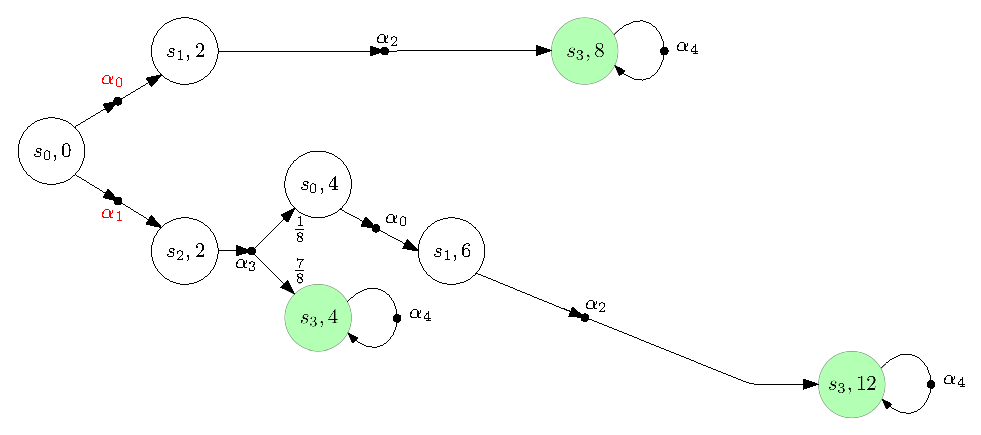
\includegraphics[width=0.8\linewidth]{resources/main-example-unfoldingA}
  \caption{$\mathcal{M}_{l_1}$ limited to safe actions of $\mathbb{A}$}
  \label{safe_actions}
\end{figure}
In $\mathcal{M}_{l_1}^\mathbb{A}$, we can easily compute the minimal expected cost-to-target for $T_{l_1}$ since there is actually only one nondeterministical choice in $\mathcal{M}_{l_1}^\mathbb{A}$: either the strategy chooses $\alpha_0$ for the state $(s_0, 0)$ and the expected cost-to-target corresponding to this choice is $8$, or it chooses $\alpha_1$ (we denote this strategy by $\sigma^{\alpha_1}$), and the expected cost-to-target is
\[
  \mathbb{E}^{\sigma^{\alpha_1}}_{(s_0, 0)}(\TS^{T_{l_1}}) = \frac{7}{8} \cdot 4 + \frac{1}{8} \cdot 12 = 5.
\]
Thus, the minimal expected cost from $s$ to $T$ while ensuring to reach $T$ with probability one is $5 \leq 6$, and thus the \SSPWE{} problem is solved. The optimal pure memoryless strategy $\sigma^{\alpha_1}$ in $\mathcal{M}_{l_1}^\mathbb{A}$ corresponds
in $\mathcal{M}$ to the memory strategy trying once $\alpha_1$, and then choosing $\alpha_0$ if it has failed, i.e., trying once a direct sending to the node $n_2$, and then sending the message via the intermediate node $n_1$ if it has failed.
\end{example}

\section{Percentile queries in multi-dimensional Markov decision processes}
In this section, we define some strategies allowing to deal with multiple \textit{percentile queries} in \textit{multi-dimensional Markov decision processes}.
A multi-dimensional MDP is an MDP where the weigth of each action has multiple dimensions.
Remind the \SSPP{} problem in Section \ref{vssp} from Chapter \ref{preliminaries}.
This problem actually consists in deciding the existence of a strategy satisfying one single percentile query.
We are now interested in defining a strategy solving \textit{simultaneously} multiple \SSPP{} problem on different weight dimension and for different set of target states.

\begin{definition}[\textbf{Multi-dimensional Markov decision process}]
  A $d$-dimensional MDP is a tuple $\mathcal{M}=(S, A, \Delta, w, AP, L)$ where
  \begin{itemize}
    \item $S, A, \Delta, AP, L$ are defined as for classical MDPs, and
    \item $w$ is a $d$-dimension weight function $w: A \rightarrow \mathbb{N}_0^d$.
    For $k \in \{1, \dots, d\}$, $w(\alpha)_k$ is the weight of the action $\alpha$ on the $k^\text{th}$ dimension.
  \end{itemize}
\end{definition}

\begin{example}[\textit{Multi-dimensional MDP for the wireless sensor network}]
  We update the MDP presented in Example \ref{spg-example} in order to fill in the details left open in the situation of Example \ref{main-example}.
  \begin{figure}[h]
    \centering
    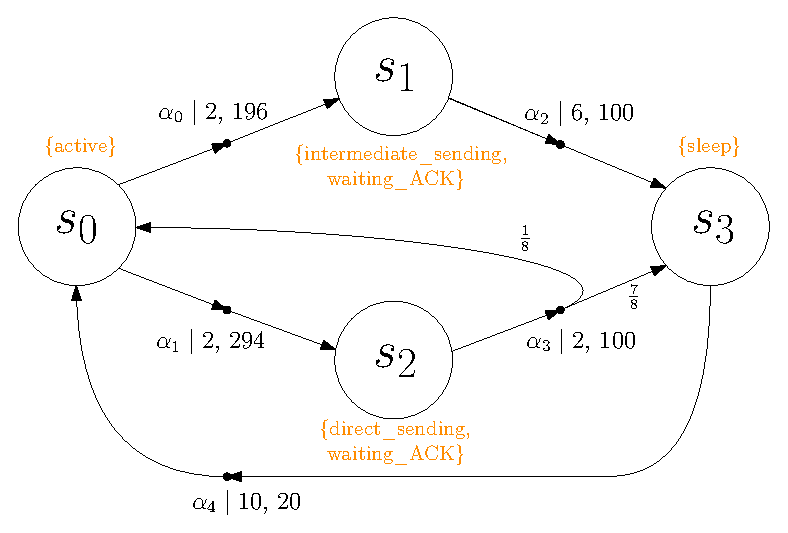
\includegraphics[width=0.6\linewidth]{resources/mdmdp2}
    \captionsetup{justification=centering}
    \caption{Multi-dimensional MDP modelling the situation of Example \ref{main-example}}
    \label{multi-mdp}
  \end{figure}
  We modify the weight function in order to support the energy cost of each action. This modification yields the MDP of Figure \ref{multi-mdp}.
  We assume here that waiting an ACK from a node uses $100$ \textit{mili Joules} ($mJ$), sending a message to $n_1$ uses $196$ $mJ$, sending a message to $n_2$ uses $294$ $mJ$, and staying in the \textit{sleep} state during $10$ $ms$ uses $20$ $mJ$.
\end{example}

\begin{remark}[\textit{Truncated sum in a multi-dimensional MDP}]
  The truncated sum function $\TS$ must be slightly modified to handle multidimensional MDPs.
  Indeed, let $\mathcal{M}$ be a $d$-dimensional MDP with state space $S$ and weight function $w$.
  We denote by $\TS^T_{k}$ the truncated sum up to $T$ on the $k^\text{th}$ dimension, with $k \in \{1, \dots, d\}$.
  More formally, let $\pi = s_0 \xrightarrow{\alpha_1} s_1 \xrightarrow{\alpha_2} s_2 \xrightarrow{\alpha_3} \dots \in Paths(s)$ be a path of $\mathcal{M}$ starting from $s \in S$,
  \[
  \TS^T_k(\pi) = \begin{cases}
    \sum_{i=1}^{n} w(\alpha_i)_k & \text{if } \forall i \in \{0, \dots, n-1\}, \, s_{i} \not\in T \, \wedge \, s_n \in T, \\
    + \infty & \text{else}.
  \end{cases}
  \]
  Furthermore, let $\sigma$ be a strategy on $\mathcal{M}$, we can define the event $\Diamond_{k: \, \leq l} \, T$ on $\sigma$-paths  starting from $s \in S$ as follows:
  \[
    \Diamond_{k:\,\leq l}\,T=\{\pi \in Paths^\sigma(s) \; | \; \TS^T_k(\pi) \leq l \}.
  \]
\end{remark}

\begin{definition}[\textbf{\SSPPQ{} problem}]
  Let $\mathcal{M}=(S, A, \Delta, w, AP, L)$ be a $d$-dimensional MDP, $s \in S$, and $q \in \mathbb{N}$ percentile constraints. These percentile constraints are described by a set of target states $T_i \subseteq S$, the dimensions $k_i \in \{1, \dots, d\}$, the cost thresholds $l_i \in \mathbb{N}$, and the probability thresholds $\alpha_i \in [0, 1] \cap \mathbb{Q}$, for each $i \in \{1, \dots, q\}$.
  The \textit{stochastic shortest path percentile queries} problem (\SSPPQ{}, for short) consists in deciding if there exists a strategy $\sigma$ such that
  \[
    \bigwedge_{i \in \{1, \dots, q \}} \mathbb{P}^\sigma_s(\Diamond_{k_i:\, \leq l_i}\, T_i) \geq \alpha_i.
  \]
\end{definition}

\begin{example}[\textit{\SSPPQ{} problem in the wireless sensor network}]
  Let $\mathcal{M}$ be the MDP of Figure \ref{multi-mdp}, modelling the situation described in Example \ref{main-example} for the node $n_0$.
  We are interested to satisfy multiple percentile queries in $\mathcal{M}$, from the state $s_0$ (i.e., the \textit{active} state of the sensor $n_0$).
  Firstly, we want to ensure with a probability of $80 \%$ that the message will be sent to the sensor $n_2$ and acknowledged within $4 \; ms$ (cf. query $\mathcal{Q}_1$). Secondly, we want to ensure with a probability of $90 \%$ that the message will be sent to the sensor $n_2$ and acknowledged with an energy cost inferior or equal than $700 \; mJ$ (cf. query $\mathcal{Q}_2$).
  \begin{align*}
    &\bigcdot\;\mathcal{Q}_1 := \,  ?\exists \sigma \;\; \mathbb{P}^{\sigma}_{s_0}(\Diamond_{1: \, \leq 4} \, \{s_3\}) \geq 0.8 \\
    &\bigcdot\;\mathcal{Q}_2 := \, ? \exists \sigma \;\; \mathbb{P}_{s_0}^{\sigma}(\Diamond_{2: \, \leq 700} \, \{s_3\}) \geq 0.9
  \end{align*}
  Let $\sigma_1$ and $\sigma_2$ be two pure memoryless strategies on $\mathcal{M}$ such that
  \begin{itemize}
    \item $\sigma_1$ corresponds to the strategy always trying a direct sending to $n_2$, and
    \item $\sigma_2$ corresponds to the strategy sending the message via $n_1$.
  \end{itemize}
  The strategy $\sigma_1$ satisfies $\mathcal{Q}_1$, but $\sigma_1$ does not satisfies $\mathcal{Q}_2$.
  Indeed, this strategy yields %on $Paths^{\sigma_1}(s_0)$
  the events
  \[\Diamond_{1:\, \leq 4}\, \{s_3\} = \Diamond_{2:\, \leq 700}\, \{s_3\} = \{ \pi \in Paths^{\sigma_1}(s_0) \; | \; s_0 %\xrightarrow{\alpha_1}
  s_2 %\xrightarrow{\alpha_3}
  s_3 %\xrightarrow{\alpha_4} \,
  \in Pref(\pi) \},\]
  because $\TS^{\{s_3\}}_1 (s_0 \xrightarrow{\alpha_1}s_2 \xrightarrow{\alpha_3}s_3 \dots) = 4 $,
  $\TS^{\{s_3\}}_2 (s_0 \xrightarrow{\alpha_1}s_2 \xrightarrow{\alpha_3}s_3 \dots) = 394 $, and
  paths of the form $s_0 \xrightarrow{\alpha_1}s_2 \xrightarrow{\alpha_3}s_0 \dots$ necessarily exceed the cost thresholds $4$ and $700$.
  Then, $\mathbb{P}_{s_0}^{\sigma_1}(\Diamond_{1:\, \leq 4}\{s_3\}) = 0.875 \geq 0.8$ and $\mathbb{P}_{s_0}^{\sigma_1}(\Diamond_{2: \, \leq 700} \, \{s_3\}) = 0.875<0.9$.
  In the same way, $\sigma_2$ satisfies $\mathcal{Q}_2$, but $\sigma_2$ does not satisfy $\mathcal{Q}_1$.
  Indeed, $\sigma_2$ yields the events
  \[
    \Diamond_{1:\, \leq 4} \, \{s_3\} = \emptyset, \text{ and }
    \Diamond_{2:\, \leq 700} \, \{s_3\} = \{\pi \in Paths^{\sigma_2}(s_0) \; | \; s_0s_1s_3 \in Pref(\pi)\},
  \]
  because all $\sigma_2$-paths starting from $s_0$ have the form $s_0\xrightarrow{\alpha_0}s_1\xrightarrow{\alpha_2}s_3\dots$, and
  $\TS^{\{s_3\}}_1(s_0\xrightarrow{\alpha_0}s_2\xrightarrow{\alpha_2}s_3\dots) = 8 > 4$, and $\TS^{\{s_3\}}_2(s_0\xrightarrow{\alpha_0}s_2\xrightarrow{\alpha_2}s_3 \dots) = 296 \leq 700$. Then,
  $\mathbb{P}_{s_1}^{\sigma_2}(\Diamond_{1:\, \leq 4}\{s_3\}) = 0 < 0.8$ and $\mathbb{P}_{s_0}^{\sigma_2}(\Diamond_{2: \, \leq 700} \, \{s_3\}) = 1 \geq 0.9$.
  \par In order to satisfy both queries at the same
  time, we will consider a finite-memory strategy
  $\sigma_{1\wedge2}$ with two modes, representing
  a \textit{compromise} between these two strategies (cf.
  Figure \ref{strat-compromise}).
  \begin{figure}[h!]
    \centering
    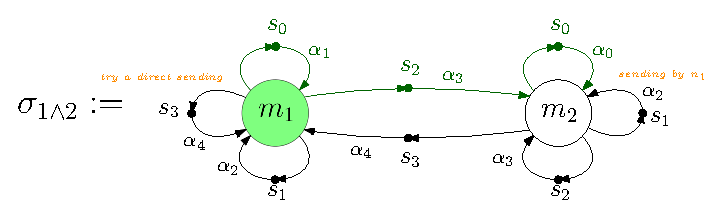
\includegraphics[width=0.7\linewidth]{resources/strategy2}
    \caption{Strategy representing a compromise between $\sigma_1$ and $\sigma_2$ on $\mathcal{M}$}
    \label{strat-compromise}
  \end{figure}
  Indeed, we assume that $\sigma_{1 \wedge 2}$ is initialised in the mode $m_1$ and first try a direct sending to $n_2$. If it fails, it then sends the message via $n_1$.
  As $\sigma_{1 \wedge 2}$ tries a direct sending to $n_2$,
    the cost of this try is $4$ $ms$, $394$ $mJ$ and succeeds with a probability $\frac{7}{8}$. If it fails, the strategy sends the message via $n_1$ and the time thresholds is exceeded.
    It does however not matter because the probability threshold is satisfied.
    In that case, the total cost of the sending is exactly $394 + 296 = 690 < 700$ $mJ$. Thus,
  \begin{itemize}
    \item $\mathbb{P}_{s_0}^{\sigma_{1 \wedge 2}}(\Diamond_{1:\, \leq 4}\, \{s_3\}) = 0.875 \geq 0.8 \implies \sigma_{1 \wedge 2} \text{ satisfies }\mathcal{Q}_1, \text{ and}$
    \item $\mathbb{P}_{s_0}^{\sigma_{1 \wedge 2}}(\Diamond_{2:\, \leq 700}\, \{s_3\}) = 1 \geq 0.9 \implies \sigma_{1 \wedge 2} \text{ satisfies }\mathcal{Q}_2.$
  \end{itemize}
\end{example}
